\documentclass[aspectratio=169]{beamer}
\usepackage{listings}

% Haskell code listings in our own style
\usepackage{listings,color}
\definecolor{lightgrey}{gray}{0.35}
\definecolor{darkgrey}{gray}{0.20}
\definecolor{lightestyellow}{rgb}{1,1,0.92}
\definecolor{dkgreen}{rgb}{0,.2,0}
\definecolor{dkblue}{rgb}{0,0,.2}
\definecolor{dkyellow}{cmyk}{0,0,.7,.5}
\definecolor{lightgrey}{gray}{0.4}
\definecolor{gray}{gray}{0.50}
\lstset{
	language        = Haskell,
	basicstyle      = \scriptsize\ttfamily,
	keywordstyle    = \color{dkblue},     stringstyle     = \color{red},
	identifierstyle = \color{dkgreen},    commentstyle    = \color{gray},
	showspaces      = false,              showstringspaces= false,
	rulecolor       = \color{gray},       showtabs        = false,
	tabsize         = 8,                  breaklines      = true,
	xleftmargin     = 8pt,                xrightmargin    = 8pt,
	frame           = single,             stepnumber      = 1,
	aboveskip       = 4pt plus 2pt,
	belowskip       = 6pt plus 2pt,
}
\lstnewenvironment{code}[0]{}{}

\title{Finite Automata in Haskell}
\author{V. Velkey, W. Vromen}
\date{\today}


\begin{document}
	\begin{frame}
		\titlepage
	\end{frame}
	\begin{frame}{Overview}
		\begin{itemize}
			\item Theory overview: DFA-s, NFA-s, $\epsilon$-NFA-s, Regular expressions
			\item DFA -s: implementation, evaluation of words
			\item NFA-s and $\epsilon$-NFA-s: implementation, evaluation
			\item Powerset construction: $\epsilon$-NFA to DFA
			\item RegExp: implementation, word generation
			\item RegExp to DFA
			\item DFA to RegExp
		\end{itemize}
		
	\end{frame}
	\begin{frame}{Theory Introduction - Regular Languages}
		\begin{itemize}
			\setlength\itemsep{2em}
			\item Regular languages: "read-only computation"
			\begin{itemize}
				\setlength\itemsep{2em}
				\item  Starting point of formal language theory
			\end{itemize}
			\item Equivalent characterisations: Finite Automata, Regular expressions
			\item Goal of project: formalise their equivalence in Haskell
		\end{itemize}
	\end{frame}
	\begin{frame}{Theory - DFA-s}
		\begin{figure}
			\centering
			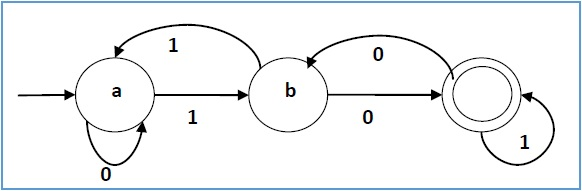
\includegraphics[scale = 0.5]{dfa_graphical_representation.jpg}
			%\caption{Example for combinatorial represenation}
			%\label{fig:my_label}
		\end{figure}
		Formal definition: $(Q_n, \Sigma, \delta_n, q_0, F_n)$
		\begin{itemize}
			\item $Q_n$ set of states
			\item $\Sigma$ alphabet
			\item $\delta_n$ transition function (between states): $\delta (\mathrm{st}, \mathrm{sym}) = \mathrm{st}' $
			\item $q_0$ start state
			\item $F_n$ set of accept states
		\end{itemize}
	\end{frame}
	\begin{frame}{Theory - NFA-s, $\epsilon$-NFA-s}
		NFA-s:
		\begin{itemize}
			\item can transition to multiple states
			\item Accept: if at least one path at accept
		\end{itemize}
		$\epsilon$-NFA-s: 
		\begin{itemize}
			\item Can transition between states without moving along the word
		\end{itemize}
		\begin{figure}
			\centering
			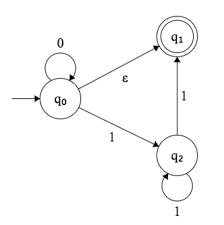
\includegraphics[scale = 0.5]{enfa.png}
			%\caption{Example for combinatorial represenation}
			%\label{fig:my_label}
		\end{figure}
	\end{frame}
	\begin{frame}{Theory - Regular expressions}
		Algebraic (recursive) way to build languages
		\begin{itemize}
			\item $\emptyset$, defines $L(\emptyset) = \emptyset$.
			\item $\epsilon$, defines $L(\epsilon) = \{\epsilon\}$
			\item $a$, defines $L(a) = \{a\}$
			\item $E\cup F$, defines $L(E\cup F) = L(E) \cup L(F)$
			\item $EF$, defines $L(E)L(F)$ (concatenation)
			\item $E^*$ defines $L(E^*) = L(E)^* = \bigcup_{n\geq 0} L(E)^n$
		\end{itemize}
	\end{frame}
	\begin{frame}{Theory - Equivalence}
		\begin{itemize}
			\setlength\itemsep{2em}
			\item For every $\epsilon$-NFA, there is an equivalent DFA (powerset construction below)
			\item For every	DFA there is an regular expression with the same language ($R_{i, j, k}$ construction below)
			\item For every RegExp, there is an $\epsilon$-NFA on the same language (regExpToENFA)
		\end{itemize}
	\end{frame}
	\begin{frame}[fragile]{DFA -s: implementation, evaluation of words}	
		Design choice: words with unknown symbols will be \textit{rejected}. 
	
	 \begin{code}
type Symbol = Char
data DFA a = DFA { states :: [a] 
	, alphabet:: [Symbol]
	, delta :: Symbol -> a -> a
	,  start:: a
	, acceptstate:: [a]}
		
evaluate:: (Eq a, Ord a) => DFA a -> String -> Bool
evaluate df st = all (`elem` alphabet df) st && -- all characters in string are in the alpahbet
		stateArr (start df) st `elem` acceptstate df where 
		  stateArr  q [] = q
		  stateArr q (x:xs) = stateArr (delta df x q) xs
	
	\end{code}
	\end{frame}
	\begin{frame}[fragile]{DFA Arbitrary}
		To generate functions: use idea from HW2
		\begin{code}
randomDelta :: (Eq a, Ord a, Arbitrary a) => [Symbol] -> [a] -> [a] -> Gen (Symbol -> a -> a)
randomDelta [] _ _ = return (const undefined)
randomDelta (sym:syms) ds ps = do 
f <- randomDelta syms ds ps
wResult <- randomFunFromTo ds ps
return $ \sy -> if sy == sym then wResult else f sy

instance Arbitrary (DFA Int) where
arbitrary = do
-- choose a set of up to 4 worlds:
sts <- (0 :) <$> sublistOf [1..3]
let sym = ['0', '1']
delt <- randomDelta sym sts sts
strt <- elements sts
accraw <-  sublistOf sts
let acc = nub (0:accraw)
return $ DFA sts sym delt strt acc
		\end{code}
	\end{frame}
	\begin{frame}[fragile]{NFA implementation}
Transitioning between lists of states: double recursion. 		
		\begin{code}
data NFA a= NFA { statesNF :: [a]
	, alphabetNF:: [Symbol]
	, deltaNF :: Symbol -> a -> [a]
	, startNF:: a
	, acceptstateNF:: [a]}
	
evaluateNF:: Eq a => NFA a-> String -> Bool
evaluateNF nf st = all (`elem` alphabetNF nf) st && -- captures elements of string in alphabet
		any (`elem` acceptstateNF nf) (stateArrNF' [startNF nf] st)  where
		  stateArrNF'  qs [] = qs
		  stateArrNF'  [] _ = []
		  stateArrNF'  [q] (x:xs) = stateArrNF' (deltaNF nf x q) xs --recursion on string
		  stateArrNF'  (q:qs) (x:xs) = stateArrNF' [q] (x : xs) `union` stateArrNF' qs (x : xs) --recursion on statespace
		\end{code}
	\end{frame}
	\begin{frame}[fragile]{$\epsilon$-NFA-s}

			 Design choice: $\epsilon$-transitions represented as list of tuple - ease with transitive closure			
		\begin{code}
data ENFA a = ENFA { statesENF :: [a]
	, alphabetENF:: [Symbol]
	, deltaENF :: Symbol -> a -> [a]
	, epTrans:: [(a, a)]
	, startENF:: a
	, acceptstateENF:: [a]}
	
rtClose:: (Eq a, Ord a) => ENFA a -> [a] -> [a]
rtClose nf qs = sort (unionL [[p | p <- statesENF nf , (q, p) `elem` trClose rcl ] | q<- qs] ) where
	rcl = refClose (statesENF nf) (epTrans nf)			
				
		\end{code}
	\end{frame}
	\begin{frame}{The powerset construction - definition}
		\begin{itemize}
			\item Take NFA $N = (Q_n, \Sigma, \delta_n, q_0, F_n)$
			\item Powerset construct: $D = (\mathcal{P}(Q_n), \Sigma, \delta, S, F_D )$
			\begin{itemize}
				\item States: subsets of $Q_n$
				\item Alphabet: same (of course)
				\item transition function: $\delta_D(R, \sigma) = \cup_{s\in R} \delta_N(s, \sigma)$
				\item Start state: singleton with previous start state
				\item Accept states: $\{R\subset Q_N \colon S\cap F_n \neq \emptyset\}$
			\end{itemize}
			\item For $\epsilon$-NFA: \\
			Similar idea, but at each step, need to take  $\epsilon$-closure at steps
				\begin{itemize}
					\item  Start state $\mathrm{ecl}(\{q_0\})$
					\item  transition function: $\delta_D(R, \sigma) = \mathrm{ecl}(\cup_{s\in R} \delta_N(s, \sigma))$
				\end{itemize}
		\end{itemize}
		\end{frame}
		\begin{frame}[fragile]{Powerset construction - implementation}
			For $\epsilon$-NFAs: 
			\begin{code}
enfaToDFA:: (Eq a, Ord a) => ENFA a -> DFA [a]
enfaToDFA (ENFA sts alph del eps strt ac) = let nf = ENFA sts alph del eps strt ac in 
cutDFA $ DFA sortedStates alph del' (rtClose nf (sort [strt])) [st | st <- sortedStates,  intersect st ac /= []] where
del' sy ls = let nf = ENFA sts alph del eps strt ac in rtClose nf ( unionL [del sy l | l <- ls] )
sortedStates = map sort $ subsequences sts
			\end{code}
			\begin{itemize}
				\item  Problem: By definition, exponential-size DFA
				\item Working with the output DFA ($~2^{19}$ states): unfeasible
				\item Workaround: cutDFA - only work with states reachable from start state
				\item  Even better: construct \textit{minimal} equivalent DFA
				\begin{itemize}
					\item Not too efficient
				\end{itemize}
			\end{itemize}
		\end{frame}
	\begin{frame}[fragile]{RegExp implementation: data type}
		\begin{code}
data RegExp = Empty | Epsilon | R [Symbol] | Union RegExp RegExp 
              | Star RegExp | Con RegExp RegExp | Plus RegExp 
  deriving (Show, Eq)
		\end{code}
	Design choices:
	\begin{itemize}
\item not split empty from non-empty expressions	
\item \texttt{Epsilon} versus \texttt{R []}
\item \texttt{R [Symbol]} versus \texttt{R Symbol} 
	\end{itemize}
For convenience:
\begin{code}
regExpUnion :: [RegExp] -> RegExp
regExpUnion = simplify . foldr Union Empty
\end{code}		
	\end{frame}	
	\begin{frame}[fragile]{Tests}
		\begin{code}
"ZeroStart accepts words starting with 0:"
+++ OK, passed 100 tests.
"ZeroStart does not accept other words:"
+++ OK, passed 100 tests.
"Powerset construction yields equivalent DFA for ENFA:"
+++ OK, passed 100 tests.
"DFA accepts words generated by the corresponding RegExp:"
+++ OK, passed 100 tests.
"DFA does not accept words generated by the RegExp corresponding to the complement DFA:"
+++ OK, passed 100 tests.
"ENFA corresponding to RegExp accepts words generated from RegExp:"
+++ OK, passed 100 tests.
"Minimize doesn't yield more states"
+++ OK, passed 100 tests.
"cutDFA dfa accepts and rejects the same as dfa"
+++ OK, passed 100 tests.
"The reverse of the reverse is isomorphic to the original"
+++ OK, passed 100 tests.
"Minimize yields an automaton that accepts and rejects the same words:"
+++ OK, passed 100 tests.
"Composition of transitions yields equivalent DFA for DFA:"
+++ OK, passed 100 tests.
\end{code}
	\end{frame}
\end{document}